\chapter{Methods in ...}

As manny other  this project developed while its was happening. In this chapter it will be explained what has been done and how it was done. Here is a short summery : 
Set up the Husky with UM7, OS1 and "Point cloud to scan". Then it has all the components needed for Nav2. 
Making husky SLAM, Navigate on pre made map, SLAM and navigation together 
Set up TurtleBot3 with namespace 
To make the TurtleBot3 flow the husky there are multiple options for this: 

\begin{description}
   \item[Mimic] Where the husky and TurtleBot3 resives the same "cmd\_vel" from either telop or Nav2 running on the husky
   \item[Time delay] It is the same as mimic but with a time delay. Husky receives "cmd\_vel" form telop or Nav2. A node called "cmd\_vel\_subpub\_v0.py" also receives "cmd\_vel" converts to tb/cmd\_vel with a time delay witch the TurtleBot3 receives. 
   \item[Nav2 API] Both husky and TurtleBot3 run Nav2, a node receives husky position and sends a "Nav2 Goal" to the TurtleBot3 behind the husky. This can be done with the Nav2 API called "BasicNavigater()" in python.
   \item[AprilTags] The tf between the husky and the TurtleBot3 will be obtained using the AprilTag system. Based on the tf the TurtleBot3 can follow the husky. 
\end{description}


\section{Husky}
\subsection{Hardware}

\subsection{Software}

\section{TurtleBot3}
\subsection{Hardware}
The TurtleBot3 started with no battery and was driven by a Raspberry Pi. The Pi was running Ubuntu Server and had an old student project saved. It had performance issues, writing in the TUI was choppy. The Pi was flashed with Ubuntu Server 20.04 in an attempt to increase the performance. This did not work, and therefor it was decided tho switch out the Pi. A Xavier was available, it is same as the Husky is using and was therefor chosen. The TurtleBot3 uses a battery similar to RC Cars, RC battery's was ordered though a local hobby store. Look at Figure \ref{fig:TB3Hardware}

\begin{figure}[H]
    \centering
    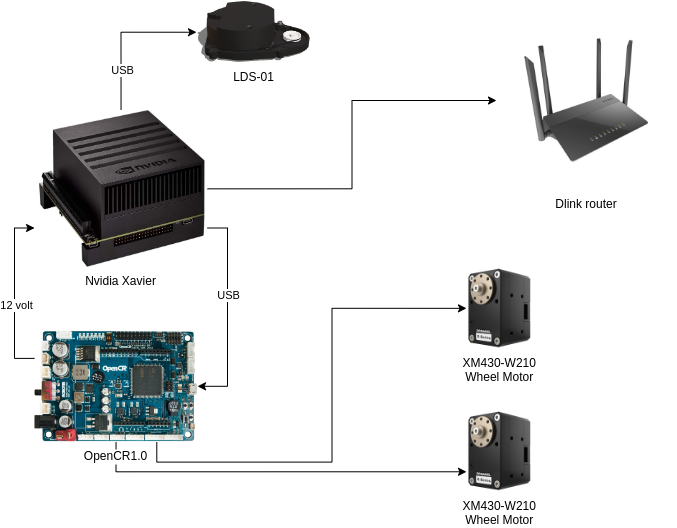
\includegraphics[width = 0.5\textwidth]{Figures/drawio/TB_HW.drawio.png}
    \caption{TurtleBot3 hardware map}
    \label{fig:TB3Hardware}
\end{figure}

\subsection{Software}
